\subsection{盒子}
\begin{enumerate}

\item 盒子的概念:盒子(box)是 \LaTeX 排版的基础。所有字符、符号甚至图表均被视为大小不一的矩形盒子。盒子是排版的最小单位,通过计算并调整盒子的位置可以使内容正确排布,从而获得合适的排版效果。

\item 盒子模型:每个盒子都是一个矩形区域,一个盒子模型有如下主要参数:

\begin{tcolorbox}[colback=white]
\centering 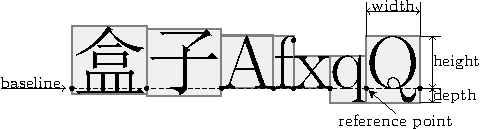
\includegraphics{./resource/tikz/box.pdf}
\end{tcolorbox}

\begin{itemize}
    \item 宽度(width):盒子的左边线与右边线的距离;
    \item 基线(baseline):基线是盒子竖直对齐的参照,当一系列盒子水平排列时,它们的基线总是对齐;
    \item 高度(height):基线与盒子的上边线的距离;
    \item 深度(depth):基线与盒子的下边线的距离;
    \item 参照点(reference point):基线与盒子的左边线的交点,也是盒子水平对齐的参照。当一系列盒子竖直排列时,它们的参照点总是对齐。
\end{itemize}

高度与深度之和是盒子的总高度。

% \item 盒子的分类:盒子主要分为三类:

% \begin{enumerate}
%     \item 普通盒子:通过输入内容直接由系统生成的盒子
%     \item 环境盒子:通过环境命令生成的盒子
%     \item 自定义盒子:通过专门的盒子命令生成的盒子
% \end{enumerate}

\item 生成盒子:\boxforcmd{\\mbox{}} 用于生成无边框盒子,参数为各种内容,也可以为空。空盒子不占宽度,可用其做水平空白命令的挡板。

\item 生成边框盒子:\boxforcmd{\\fbox{}} 用于生成边框盒子,如 \verb|\fbox{box}| 表现为 \fbox{box}

\item 盒子的尺寸调整:声明 \boxforcmdbox{\ttfamily \textbackslash fboxrule=\itshape size} 和 \boxforcmdbox{\ttfamily \textbackslash fboxsep=\itshape size} 用于设定盒子边框线的粗细(默认值是 0.4pt;当尺寸设置为 0 时,则没有边框线)和设定盒子中内容与边框线的距离(即盒子内边距,默认值是 3pt。当尺寸设置为 0 时,则边框线紧贴内容),这两个可以放在导言区,从而对整篇文档起作用。

\item 定宽盒子:\boxforcmd{\\makebox[][]{}} 用于生成一个固定宽度的无框盒子,第一个可选参数为宽度,第二个可选参数为对齐方式。对齐方式有四种 \boxforcmd{lrcs} ,分别表示左对齐、右对齐、居中对齐(默认)和两端对齐。

\item 定宽边框盒子:\boxforcmd{\\framebox} 命令相当于在 \boxforcmd{\\makebox} 生成的盒子的四周添加边框,参数用法相同。

\item 虚线盒子:\boxforpkg{dashbox} 宏包提供的 \boxforcmd{\\dbox{}} 用于生成虚线边框盒子,以及 \boxforcmd{\\dashbox} 用于生成定宽虚线盒子。如 \verb|\dbox{box}| 表现为 \dbox{box}

声明 \boxforcmdbox{\ttfamily \textbackslash dashlength=\itshape size} 和 \boxforcmdbox{\ttfamily \textbackslash dashdash=\itshape size} 分别设置虚线盒子虚部的长度和实部的长度。

\item 盒子的溢出和不足:对于一个宽度或高度固定的盒子,在正常排版时内容应当位于盒子内部,如果内容超出了盒子的范围,会发生内容的溢出(overfull)。溢出会发生内容的越位,可能造成覆盖或丢失等问题,例如:

\begin{tcolorbox}[sidebyside]
\begin{lstlisting}
\framebox[10ex][l]{overfull box} covered some content
\end{lstlisting}

\tcblower
\raggedleft
\framebox[10ex][l]{\mbox{overfull box}} covered some content
\end{tcolorbox}

如果盒子的宽度太大且内容不足,而盒子又必须被填满,此时就会发生内容的不足(underfull)。这经常发生于两端对齐的情况,此时内容间就会强行添加额外的空白来填充宽度。

\item 升降盒子:命令 \boxforcmdbox{\ttfamily \textbackslash raisebox\{{\itshape raise}\}[{\itshape height}][{\itshape depth}]\{{\itshape text}\}} 可以使盒子对象在垂直方向上升或下降。

必选参数 {\ttfamily\itshape raise} 决定了内容在垂直方向上移动的距离;可选参数 {\ttfamily\itshape height} 和 {\ttfamily\itshape depth} 决定了移动后盒子的实际高度与深度。如果忽略可选参数,移动后盒子的尺寸将自动适应内容;如果指定了可选参数,则盒子的实际尺寸与内容无关,可能造成溢出。

升降盒子实际上是盒子的嵌套,它用一个新的盒子套住现有内容,让现有内容在其中上下移动,新盒子的尺寸由可选参数决定。例如:

\begin{tcolorbox}[sidebyside, righthand width=0.33\linewidth]
\begin{lstlisting}
\fbox{\raisebox{18pt}{\dbox{box}}}
\fbox{\raisebox{-14pt}{\dbox{box}}}
\fbox{\raisebox{14pt}[18pt]{\dbox{box}}}
\fbox{box}
\fbox{\raisebox{20pt}[16pt]{\dbox{box}}}
\fbox{\raisebox{-18pt}[16pt][10pt]{\dbox{box}}}
\end{lstlisting}

\tcblower
\fboxrule=0.2pt \fboxsep=0pt
\Large

\fbox{\raisebox{18pt}{\dbox{box}}}
\fbox{\raisebox{-14pt}{\dbox{box}}}
\fbox{\raisebox{14pt}[18pt]{\dbox{box}}}
\fbox{box}
\fbox{\raisebox{20pt}[16pt]{\dbox{box}}}
\fbox{\raisebox{-18pt}[16pt][10pt]{\dbox{box}}}
\end{tcolorbox}

\item 零尺寸盒子:当用盒子命令生成了一个零尺寸的盒子以后,将它放在任意位置均不会影响其它内容的排版,且移动的基准点为原先盒子的参考点,可以在不破坏文档布局的情况下调整元素。

\begin{tcolorbox}[sidebyside, righthand width=0.4\linewidth]
\begin{lstlisting}
\raisebox{10pt}[0pt][0pt]{ \hspace{-30pt} 
    \makebox[0pt]{zero box} } and ...
\end{lstlisting} 

\tcblower

\raisebox{10pt}[0pt][0pt]{\LARGE
    \hspace{-30pt}\makebox[0pt]{zero box}
} and following content
\end{tcolorbox}

\item 行盒子:使用以上命令生成的盒子均是行盒子,它们的特点是只占一行,如果内容宽度超出了盒子或文档宽度也不会自动换行,而是会溢出。但是行盒子的高度和深度会随着内容自动调整。

\begin{tcolorbox}[sidebyside]
\begin{lstlisting}
\framebox[6em]{ \dbox{  
  This is a {\LARGE long} long 
  \raisebox{-10pt}{long} long line }}
\end{lstlisting} 

\tcblower

\framebox[6em][l]{ \dbox{
    This is a {\LARGE long} long \raisebox{-10pt}{long} long line
    } 
}
\end{tcolorbox}

\item 段落盒子:使用 \boxforcmdbox{\ttfamily \textbackslash parbox[{\itshape position}][{\itshape height}][{\itshape inner-pos}]\{{\itshape width}\}\{{\itshape text}\}} 可以得到段落盒子,段落盒子的内容将根据宽度自动做断行处理。

必选参数 {\ttfamily\itshape width} 决定段落盒子的宽度。可选参数 {\ttfamily\itshape position} 决定段落盒子的竖直对齐方式 \boxforcmd{tcb};{\ttfamily\itshape height} 可以手动指定内容的高度;{\ttfamily\itshape inner-pos} 决定盒子中内容的水平对齐方式 \boxforcmd{tcbs} 。例如:

\begin{tcolorbox}[sidebyside, righthand width=0.45\linewidth]
\begin{lstlisting}
\fbox{\LARGE parbox:} 
\fbox{\parbox[b]{14em}{a parbox is ...}}
\end{lstlisting} 

\tcblower

\fbox{\LARGE parbox:} \fbox{\parbox[b]{14em}{a parbox is a box whose contents are created in paragraph mode}}
\end{tcolorbox}

\item 小页环境:使用 \boxforenv{minipage} 可以得到小页环境。小页环境和段落盒子差不多,且参数的用法都基本一致。小页环境更适合包含大量图表等内容时使用。

\item 缩放盒子:需要 \boxforpkg{graphicx} 宏包支持,命令 \boxforcmdbox{\ttfamily \textbackslash scalebox\{\textit{h-scale}\}[\textit{v-scale}]\{\textit{text}\}} 可以缩放一个盒子,水平缩放系数 {\ttfamily\itshape h-scale} 为必选参数,竖直缩放系数 {\ttfamily\itshape v-scale} 为可选参数。缩放系数设为 \verb|1| 表示不缩放,设为负值表示反向缩放,例如:

\begin{tcolorbox}[sidebyside]
\begin{lstlisting}
\makebox[0pt][l]{mirror$\Omega$}%
\scalebox{1}[-1]{mirror$\Omega$}
\end{lstlisting}

\tcblower
\Large
\makebox[0pt][l]{mirror$\Omega$}%
\color{gray!50}\scalebox{1}[-1]{mirror$\Omega$}
\end{tcolorbox}

\item 变形盒子:需要 \boxforpkg{graphicx} 宏包支持,命令 \boxforcmdbox{\ttfamily \textbackslash resizebox\{\textit{h-length}\}\{\textit{v-length}\}\{\textit{text}\}} 和带星号的命令 \newline \boxforcmdbox{\ttfamily \textbackslash resizebox*\{\textit{h-length}\}\{\textit{v-length}\}\{\textit{text}\}} 可以变形盒子。必选参数 {\ttfamily\itshape h-scale} 代表变形后的宽度;另一个必选参数 {\ttfamily\itshape v-scale} 对普通的 \verb|\resizebox| 来说代表变形后的高度,对带星号的 \verb|\resizebox*| 来说代表变形后连同深度的总高度。

在变形参数内可以使用单个感叹号 \boxforcmd{!} 表示保持原有宽高不变,也可以使用负值按相反方向缩放。

\item 旋转盒子:需要 \boxforpkg{graphicx} 宏包支持,命令 \boxforcmdbox{\ttfamily \textbackslash rotatebox[\textit{origin}=...,\textit{x}=...,\textit{y}=...,\textit{units}=...]\{\textit{angle}\}\{\textit{text}\}} 可以旋转一个盒子,必选参数 {\ttfamily\itshape angle} 指定旋转角度,顺时针为负。

\begin{tcolorbox}[sidebyside, sidebyside align=top, colback=white, lefthand width=0.6\linewidth]
    
    可选参数中的 {\ttfamily\itshape origin} 决定旋转中心,可用值如左图所示。
    
    \vphantom{\Huge Q}\verb|tcBb| 分别位于盒子顶部、中心线、基线和底部。

    \vphantom{\Huge Q}也可以换用可选参数中的 {\ttfamily\itshape x,y} ,根据盒子参考点通过坐标的方式确定旋转中心。
    
    \tcblower
    
    \raisebox{-7em}{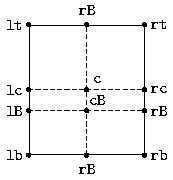
\includegraphics{./resource/tikz/rotate-origin.pdf}}

\end{tcolorbox}

可选参数中的 {\ttfamily\itshape units} 确定旋转角的单位,默认为角度。设置 \verb|units=-360| 表示以度为单位且旋转正向为顺时针;设置 \verb|units=6.283185| 表示以弧度为单位且旋转正向为逆时针等。

\begin{tcolorbox}[sidebyside, righthand width=0.3\linewidth]
\begin{lstlisting}
$\pi$ \rotatebox{45}{$\pi$} \rotatebox{90}{$\pi$}
\makebox[0pt]{\rotatebox[origin=c]{30}{\dag}}\,%
\makebox[0pt]{\rotatebox[origin=c]{-30}{\dag}}
\end{lstlisting}

\tcblower

\Large
$\pi$ \rotatebox{45}{$\pi$} \rotatebox{90}{$\pi$}
\Huge
\makebox[0pt]{\rotatebox[origin=c]{30}{\dag}}\,%
\makebox[0pt]{\rotatebox[origin=c]{-30}{\dag}}
\end{tcolorbox}

\item 花哨盒子:\boxforpkg{fancybox} 宏包提供了一系列带有花哨边框盒子的命令,包括 \boxforcmd{\\shadowbox{}} 生成 \shadowbox{阴影盒子} ,\boxforcmd{\\doublebox{}} 生成 \doublebox{双线盒子} ,\boxforcmd{\\ovalbox{}} 生成 \ovalbox{圆角盒子} ,\boxforcmd{\\Ovalbox{}} 生成 \Ovalbox{粗圆角盒子} 。

圆角盒子可以使用声明 \boxforcmd{\\cornersize{}} 和 \boxforcmd{\\cornersize*{}} 修改圆角直径,前者的参数是相对盒子宽或高的比例,后者的参数是绝对长度。例如,声明 \boxforcmd{\\cornersize{1}} 会使后续的圆角盒子变成{\cornersize{1}\ovalbox{半圆盒子}}。

\item 矩形块:\boxforcmd{\\rule[]{}{}} 命令可以创建一个填充的矩形块一样的符号,两个必选参数是矩形块的宽和高,可选参数是矩形块竖直升降的距离。

例如,\boxforcmd{\\rule{10pt}{12pt}} 创建的矩形块为 \rule{10pt}{12pt} ,\boxforcmd{\\rule[-2pt]{3em}{0.5pt} } 创建的矩形块为 \rule[-2pt]{3em}{0.5pt} 

\end{enumerate}
